% !TEX root=../main.tex
\section{Causal Inference-Based Root Cause Analysis}\label{sec:methodology}

In this section, we propose a novel method named \textit{CIRCA}.
We first present a structural way to determine the parents $\mathbf{Pa}(V_{i})$ for each metric $V_{i}$ based on system architecture.
CIRCA adopts \textit{regression-based hypothesis testing} (RHT) to deal with the incomplete distribution of faulty data.
To address the challenge of the incomplete distribution of fault-free data, CIRCA adjusts the anomaly score for suspicious metrics based on their descendants in the CBN.

\subsection{Structural Graph Construction}

We propose the \textit{structural graph} (SG) as the CBN for OSS.
SG combines the system architecture knowledge with a set of assumptions, which may not suit domains other than OSS.
We first classify monitoring metrics into four dimensions, named \textit{meta metric}s.
Several causal assumptions among those four kinds of meta metrics provide the building blocks of an SG.
% We first recognize four measurement dimensions (\textit{meta metric}s) of a computing process.
% The assumptions among those four kinds of meta metrics provide the building blocks of an SG.
We further extend the system with the architecture of components to construct a graph at the meta metric level, named a \textit{skeleton}.
Finally, we plug monitoring metrics into the corresponding meta metric to obtain the SG.
% Finally, we fulfill the skeleton with monitoring metrics to obtain the SG, replacing the corresponding meta metric.
\algref{alg:structural-graph-construction} summarizes the overall procedure.

\subsubsection{Meta Metrics}

In general, a service takes \textit{input} and produces \textit{output}.
Each request lasts for some \textit{time} and consumes some \textit{resources}.
We take those dimensions as four \textit{meta metrics} of a service, named after the four golden signals in site reliability engineering~\cite{Beyer:2016}.
\textit{Traffic}, \textit{Errors}, and \textit{Latency} measure the distribution of input, output, and processing time, respectively.
We classify other monitoring metrics as resource consumption, denoted as \textit{Saturation}.
% For example, the CPU usage will be classified as Saturation, describing a resource (the CPU device).

We assign directions for the relations among these four meta metrics in \figref{fig:tsel}.
As the start of a request, \textit{Traffic} is assumed to be the cause of all other three meta metrics, while \textit{Errors} (the end of a request) are taken as the effect of others.
% The edge from \textit{Saturation} to \textit{Latency} encodes the queuing phenomenon, \textit{i.e.}, resource consumption will not postpone a request until some kinds of resources become the bottleneck.
The edge from \textit{Saturation} to \textit{Latency} encodes our preference on the former, as resource consumption is one of the common considerations for large latency in OSS~\cite{Gan:2021}.

\begin{figure}[htb]
	\subfigure[Causal assumptions within a service]{\label{fig:tsel}
		\centering
		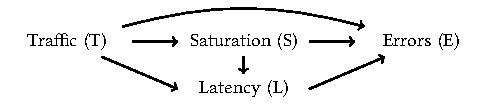
\includegraphics{img/tsel}
	} \\
	\subfigure[
	    The skeleton of one web service (WEB) with its dependent database (DB).
	    We plug DB's meta metrics into the \textit{Saturation} of WEB.
	]{\label{fig:tsel-extend}
		\centering
		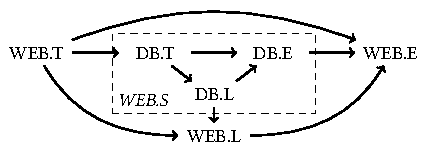
\includegraphics{img/tsel-extend}
	}
% Following is compatible to the package subcaption
% 	\begin{subfigure}{\columnwidth}
% 		\centering
% 		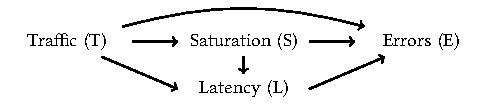
\includegraphics{img/tsel}
% 		\caption{Causal assumptions within a service}\label{fig:tsel}
% % 		\caption{within a web service}\label{fig:tsel}
% 	\end{subfigure}

% 	\begin{subfigure}{\columnwidth}
% 		\centering
% 		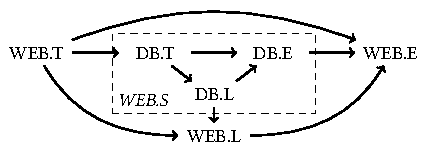
\includegraphics{img/tsel-extend}
% 		\caption{
% 		    The skeleton of one web service (WEB) with its dependent database (DB).
% 		    We plug DB's meta metrics into the \textit{Saturation} of WEB.
% 		}\label{fig:tsel-extend}
% % 		\caption{between one web service (WEB) and its dependency database(DB), fulfilling a resource (DB) with its meta metrics}\label{fig:tsel-extend}
% 	\end{subfigure}
	\caption{Causal assumptions among meta metrics}
	\Description{
		\textit{Traffic} is assumed as the cause of \textit{Saturation}, \textit{Latency}, and \textit{Errors}.
		\textit{Saturation} is assumed as the cause of \textit{Latency} and \textit{Errors}.
		\textit{Latency} is assumed as the cause of \textit{Errors}.
	}
\end{figure}

\subsubsection{Skeleton with Architecture Extension}

A complex OSS system will invoke multiple services to process one single request.
Meanwhile, there will be multiple components for monolithic OSS.
% or instructions for a function
Based on the architecture knowledge encoded in the call graph, we construct the \textit{skeleton} among meta metrics of the system and all its dependent services.
For a web service (WEB) and its database (DB) shown in \figref{fig:tsel-extend}, we take DB as a resource of WEB.
The part of WEB's Saturation that measures DB will be extended into DB's meta metrics, which inherit the relations between WEB's Saturation and other meta metrics of WEB.
The extension will be applied to each service in the call graph.
In summary, we introduce three more causal assumptions between a service and its dependent ones.

\begin{itemize}
	\item The caller's \textit{Traffic} influences the callees' \textit{Traffic};
	\item The callees' \textit{Latency} contributes to the caller's \textit{Latency};
	\item The caller's output is calculated based on the callees' output.
\end{itemize}

\subsubsection{Monitoring Metric Plugging-in}

Finally, we plug monitoring metrics in meta metrics to obtain the SG.
A mapping is required to describe which dimension of which service each monitoring metric measures.
There can be some meta metrics that do not have any monitoring metrics.
For example, the common measurement for memory is just usage (\textit{Traffic}), while the speed (\textit{Latency}) is unavailable.
Moreover, one monitoring metric can be derived from multiple meta metrics.
For example, \textit{DB access per request} is calculated by the Traffic of both a web service and a database.

\algref{alg:structural-graph-construction} describes the plugging-in process after skeleton construction.
SG links monitoring metrics from one meta metric to its children (Line \ref{line:add-edges-parent2child}).
Monitoring metrics that are derived from multiple meta metrics may introduce self-loop.
To avoid such cycles, the monitoring metric for the last meta metric in topological order will be taken as the common effect of other meta metrics (from Line \ref{line:deal-with-multi-corresponding:start} to Line \ref{line:deal-with-multi-corresponding:end}).
Moreover, meta metrics measuring the dimension of \textit{Errors} will be accumulated for descendants (Line \ref{line:accumulate-error}), as broken data may not be validated in time.

During the process, an empty meta metric will gather the monitoring metrics of its parents for its children (Line \ref{line:gather-metrics-for-children}).
Consider a meta metric ($V_{i}^{m}$), one of its parents without monitoring ($V_{j}^{m}$), and their structural equations ($f_{i}^{m}$ and $f_{j}^{m}$).
We can substitute $f_{j}^{m}$ for unobserved $V_{j}^{m}$ in $f_{i}^{m}$, as shown in \eqnref{eqn:scm-substitute-variable}.
Both the parents of $V_{j}^{m}$ and those of $V_{i}^{m}$ (except $V_{j}^{m}$) show as the parameters of $f_{i}^{m \prime}$, which is the reason behind Line \ref{line:gather-metrics-for-children}.

\begin{equation}\label{eqn:scm-substitute-variable}
	\begin{aligned}
		v_{i}^{m} & = f_{i}^{m}\left(
		f_{j}^{m}\left(\mathbf{pa}_{\mathcal{G}_{skel}}(V_{j}^{m}), \mathbf{u}_{j}^{m}\right),
		\mathbf{pa}_{\mathcal{G}_{skel}}(V_{i}^{m}) \setminus \{v_{j}^{m}\}, \mathbf{u}_{i}^{m}
		\right) \\
		& = f_{i}^{m \prime}\left(
		\mathbf{pa}_{\mathcal{G}_{skel}}(V_{j}^{m}),
		\mathbf{pa}_{\mathcal{G}_{skel}}(V_{i}^{m}) \setminus \{v_{j}^{m}\},
		\mathbf{u}_{i}^{m}, \mathbf{u}_{j}^{m}
		\right)
	\end{aligned}
\end{equation}

\begin{algorithm}[tb]
	\caption{Structural Graph Construction}\label{alg:structural-graph-construction}
	\begin{algorithmic}[1]
		\REQUIRE $\mathcal{G}_{c}$, the call graph; $\mathbf{h} : \mathbf{V}^{m} \to 2^{\mathbf{V}}$, the mapping from meta metrics $\mathbf{V}^{m}$ to monitoring metrics
		\STATE $\mathcal{G}_{s} \gets$ initial the structure graph
%		\STATE $\mathbf{h}^{\prime}: \mathbf{V}^{m} \to 2^{\mathbf{V}}$ will be an updated mapping
%		\STATE $\mathbf{r}: \mathbf{V} \to 2^{\mathbf{V}^{m}}$ records the references $\{V_{j}^{m} \mid V_{i} \in \mathbf{h}(V_{j}^{m})\}$ for each monitoring metric $V_{i}$
		\STATE $\mathcal{G}_{skel} \gets$ construct the skeleton based on $\mathcal{G}_{c}$
		\FORALL{$V_{i}^{m} \in \mathbf{V}^{m}$ in a topological order from $\{V_{j}^{m} \mid \lvert \mathbf{Pa}_{\mathcal{G}_{skel} }(V_{j}^{m}) \rvert = 0 \}$}
%			\STATE{$\mathbf{Q}_{i} \gets \bigcup_{V_{j}^{m} \in \mathbf{Pa}_{\mathcal{G}_{skel} }(V_{i}^{m})}\mathbf{h}^{\prime}(V_{j}^{m})$}
			\STATE{$\mathbf{Q}_{i} \gets$ Collect monitoring metrics of $\mathbf{Pa}_{\mathcal{G}_{skel} }(V_{j}^{m})$}
%			\STATE{$\mathbf{C}_{i} \gets \mathbf{h}(V_{i}^{m})$}
			\STATE{$\mathbf{C}_{i} \gets$ Collect monitoring metrics of $V_{i}^{m}$}
			\FOR{$V_{j} \in \mathbf{h}(V_{i}^{m})$}\label{line:deal-with-multi-corresponding:start}
%				\IF{$\lvert \mathbf{r}(V_{j}) \rvert > 1$}
				\IF{$V_{j}$ is mapped to multiple meta metrics}
					\STATE{$\mathbf{C}_{i} \gets \mathbf{C}_{i} \setminus \{V_{j}\}$}
					\COMMENT{Prevent self loop of $V_{j}$}
%					\IF{$V_{i}^{m}$ is the last meta metric in $\mathbf{r}(V_{j})$}
					\IF{$V_{j}$ is visited for the last time}
%						\STATE{Add edges from $\bigcup_{V_{k}^{m} \in r(V_{j}), i \neq k}\mathbf{h}^{\prime}(V_{k}^{m})$ to $V_{j}$ in $\mathcal{G}_{s}$}
						\STATE{Add edges from the corresponding meta metrics of $V_{j}$ other than $V_{i}^{m}$ to $V_{j}$ in $\mathcal{G}_{s}$}
						\STATE{$\mathbf{Q}_{i} \gets \mathbf{Q}_{i} \cup \{V_{j}\}$}
						\COMMENT{Take it as the proxy of others}
					\ENDIF
				\ENDIF
			\ENDFOR\label{line:deal-with-multi-corresponding:end}
			\COMMENT{Deal with monitoring metrics that are derived from multiple meta metrics}
			\STATE{Add edges from $\mathbf{Q}_{i}$ to $\mathbf{C}_{i}$ in $\mathcal{G}_{s}$}\label{line:add-edges-parent2child}
			\IF{$V_{i}^{m}$ represents Errors}
%				\STATE{$\mathbf{C}_{i} \gets \mathbf{C}_{i} \cup \bigcup_{V_{j}^{m}}\mathbf{h}^{\prime}(V_{j}^{m})$, where $V_{j}^{m} \in \mathbf{Pa}_{\mathcal{G}_{skel} }(V_{i}^{m})$ and $V_{j}^{m}$ also represents Errors}\label{line:accumulate-error}
				\STATE{Update $\mathbf{C}_{i}$ with monitoring metrics from the Errors-representing meta metrics in $\mathbf{Pa}_{\mathcal{G}_{skel} }(V_{j}^{m})$}\label{line:accumulate-error}
			\ENDIF
			\COMMENT{Transfer Errors}
			\IF{$\mathbf{C}_{i}  = \emptyset$}
%				\STATE{$\mathbf{h}^{\prime}(V_{i}^{m}) \gets \mathbf{Q}_{i}$}\label{line:gather-metrics-for-children}
				\STATE{$\mathbf{h}(V_{i}^{m}) \gets \mathbf{Q}_{i}$}\label{line:gather-metrics-for-children}
				\COMMENT{Gather monitoring metrics for children}
			\ELSE
%				\STATE{$\mathbf{h}^{\prime}(V_{i}^{m}) \gets \mathbf{C}_{i}$}
				\STATE{$\mathbf{h}(V_{i}^{m}) \gets \mathbf{C}_{i}$}
			\ENDIF
		\ENDFOR
		\RETURN $\mathcal{G}_{s}$
	\end{algorithmic}
\end{algorithm}

\subsection{Regression-based Hypothesis Testing}

% The understanding of $P_{\mathbf{m}}$ is limited due to the requirement to mitigate the failure as soon as possible.
The understanding of $P_{\mathbf{m}}$ is restricted by mitigating the failure as soon as possible.
Instead of comparing two distributions directly, we reformulate the \nameref{thm:rc-criterion} as hypothesis testing with the following null hypothesis ($\mathbf{H}_{0}$) for each metric $V_{i}$.
% Whether the value comes from an expected distribution can be measured by probability density (probability) for a continuous (discrete) metric.
% We should reject $\mathbf{H}_{0}$ if the probability density (probability) of the observation is zero.

\begin{description}
	\item[$\mathbf{H}_{0}$]  $V_{i}$ is not an indicator of the root cause, \textit{i.e.}, $$V_{i}^{(t)} \sim \mathcal{L}_{1}\left(V_{i}^{(t)} \mid \mathbf{pa}^{(t)}(V_{i})\right)$$
\end{description}

We utilize the regression technique to calculate the expected distribution $\mathcal{L}_{1}\left(V_{i}^{(t)} \mid \mathbf{pa}^{(t)}(V_{i})\right)$.
A regression model is trained for each variable with data before the fault is detected, performing as a proxy of the corresponding structural equation.
Let $\bar{v}_{i}^{(t)}$ be the regression value for $v_{i}^{(t)}$.
Assuming that the residuals follow an \textit{i.i.d.} normal distribution $N(\mu_{\epsilon,i}, \sigma_{\epsilon,i})$, \eqnref{eqn:anomaly-score:point} measures to what extent a new datum $v_{i}^{(t)}$ deviates from the expected distribution, denoted as $a_{V_{i}}^{(t)}$.
\eqnref{eqn:anomaly-score} further aggregates $a_{V_{i}}^{(t)}$ for all the available data during the abnormal period as the anomaly score of $V_{i}$.

\begin{equation}\label{eqn:anomaly-score:point}
	a_{V_{i}}^{(t)} = \left|\frac{\left(v_{i}^{(t)} - \bar{v}_{i}^{(t)}\right) - \mu_{\epsilon,i}}{\sigma_{\epsilon,i}}\right|
\end{equation}

\begin{equation}\label{eqn:anomaly-score}
	s_{V_{i}} = \max_{t} a_{V_{i}}^{(t)}
\end{equation}

\subsection{Descendant Adjustment}
% \nxh{better clarify the logic of this paragraph.}
There will be bias in the regression results due to a poor understanding of $\mathcal{L}_{1}$. 
% Inspired by the common queuing phenomenon in an online service system, we adjust the anomaly score of one metric with those of its descendants.
% For example, reducing traffic or supplementing resources is actionable to restore the low latency.
% Hence, we prefer to assign higher scores for traffic and resource utilization (the parents of latency in the CBN) than latency's score.
We adjust the anomaly score of one metric with those of its descendants.
Our intuition is that when both a metric and one of its parents in the CBN is abnormal, we prefer the latter.
For example, supplementing extra resources is an actionable mitigation method to restore the low latency.
Hence, we assign a higher score for resource utilization (the parents of latency in the CBN) than latency's score.

We summarize the adjustment in \algref{alg:descendant-adjaustment}.
The children of a metric $V_{i}$ are first considered (Line \ref{line:children:adjustment}).
We exclude some metrics ($\{V_{i} \mid s_{V_{i}} < 3\}$) from the root cause indicators, so called the \textit{three-sigma rule of thumb}.
As the failure propagates through them, those metrics will gather anomaly scores from children for the candidate root cause in their ancestors (Line \ref{line:children:propagate}).
Finally, the anomaly score of $V_{i}$ ($s_{V_{i}}$) will increase by the maximum of descendants' scores just mentioned (Line \ref{line:children:aggregate}).

\begin{algorithm}[tb]
	\caption{Descendant Adjustment}\label{alg:descendant-adjaustment}
	\begin{algorithmic}[1]
		\REQUIRE $\mathbf{s}$, anomaly scores by \eqnref{eqn:anomaly-score}
% 			$\tau \gets 3$, the threshold to estimate whether the failure just propagates through a metric
		\STATE $S \gets$ a mapping from $V_{i}$ to the anomaly scores $S(V_{i})$ that may be the direct effect of $V_{i}$
		\FOR{$V_{i} \in \mathbf{V}$ in a topological order from $\{V_{j} \mid \lvert \mathbf{Ch}(V_{j}) \rvert = 0$\}}
			\STATE $S(V_{i}) \gets \{s_{V_{j}} \mid V_{j} \in \mathbf{Ch}(V_{i})\}$\label{line:children:adjustment}
			\FOR{$V_{j} \in \mathbf{Ch}(V_{i})$}
				\IF{$s_{V_{j}} < 3$}
					\STATE{$S(V_{i}) \gets S(V_{i}) \cup S(V_{j})$}\label{line:children:propagate}
				\ENDIF
			\ENDFOR
		\ENDFOR
		\COMMENT{Collect direct effects}
		\FOR{$V_{i} \in \mathbf{V}$}
			\IF{$s_{V_{j}} \ge 3$}
				\STATE{$s_{V_{i}}^{\prime} \gets s_{V_{i}} + \max( S(V_{i}) )$}\label{line:children:aggregate}
				\COMMENT{Adjust based on descendants}
			\ENDIF
		\ENDFOR
		\RETURN $\mathbf{s}^{\prime}$, the adjusted anomaly scores
	\end{algorithmic}
\end{algorithm}
